\chapter{Recherche dichotomique d'un élément dans un tableau}

\section{Description de l'objectif de l'algorithme}
En informatique, un tableau est une structure de données représentant une séquence finie d'éléments défini par un index représentant sa position au sein du tableau nous permettant d'y accéder. C'est un type de conteneur que l'on retrouve dans un grand nombre de langages de programmation et est l'un des plus utilisés du de sa simplicité.
\par
Les données du tableau étant accessible individuellement il est nécessaire de faire une recherche lorsque l'on souhaite accéder a une valeur spécifique du tableau cependant lorsque la taille de la structure est grande il devient difficile d'y accéder efficacement, c'est pour cela que de nombreux algorithmes ont été conçu afin d'optimiser cette tache est l'un de ses algorithmes les plus performants est celui de la recherche dichotomique.
\par
La recherche dichotomique ou recherche par dichotomie, est un algorithme de recherche pour trouver la position d'un élément dans un tableau. La seule condition a son application étant que le tableau soit trie, il est utilisable dans de nombreuses problématiques. Son principe consiste comparer l'élément avec la valeur de la case au milieu du tableau, si les valeurs sont égales, on met fin à l'exécution, sinon si la valeur recherchée est inférieur à la valeur de la case au milieu, on recommence dans la moitié du tableau contenant les valeurs plus petites que celle située au milieu du tableau et dans le cas contraire on prend la moitie contenant les valeurs supérieures, et ceci jusqu'à avoir trouvé la valeur souhaite ou avoir un sous tableau n'ayant qu'une seule valeur empêchant de continuer la recherche dans le cas ou la valeur n'existe pas dans le tableau. (voir Figure \ref{fig:exp_dico}).

\begin{figure}[H]
    \centering
        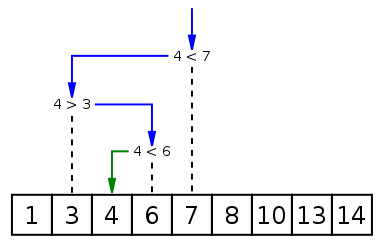
\includegraphics[scale=1.0]{./ressources/Binary_search_into_array.png}
        \caption{Exemple graphique d'une recherche dichotomique}
    \label{fig:exp_dico}
\end{figure}

\section{Fonctionnement de l'algorithme}
Il nous est possible de distinguer 2 étapes distinctes et essentiels au bon déroulement de cet algorithme la première étant le trie du tableau, car comme précisé précédemment la recherche par dichotomie nécessite que le tableau soit trié et ne pouvant pas garantir de recevoir un tableau trié en entrée il est nécessaire de le trier au préalable avant de commencer le recherche afin de pouvoir le plus de cas que possible, par la suite la seconde étape consiste à appliquer la recherche dichotomique.

\subsection{Tri du tableau}
Dans cette partie, on applique un tri ascendant sur tableau et pour cela nous appliquons l'algorithme de Tri Fusion.
\par
Le tri par fusion aussi appeler tri dichotomique est un exemple classique d'algorithme de division pour régner. L'opération principale de l'algorithme est la fusion, qui consiste à réunir deux listes triées en une seule. L'efficacité de l'algorithme vient du fait que deux listes triées peuvent être fusionnées en temps linéaire (voir Figure \ref{fig:tri_dico}). On peut résumer son fonctionnement en deux étapes :
\begin{enumerate}
  \item Divisez la liste non triée en sous-listes jusqu'à ce qu'il y ait N sous-listes avec un élément dans chacune (N est le nombre d'éléments dans la liste non triée).
  \item Fusionnez les sous-listes deux à la fois pour produire une sous-liste triée, répétez cette opération jusqu'à ce que tous les éléments soient inclus dans une seule liste.
\end{enumerate}

\begin{figure}[H]
    \centering
        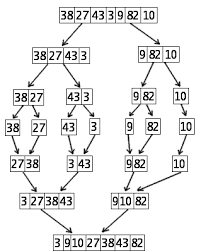
\includegraphics[scale=1.0]{./ressources/trifusion.png}
        \caption{Exemple graphique d'un tri dichotomique}
    \label{fig:tri_dico}
\end{figure}
\par
Nous pouvons le représenter via le pseudo code suivant :

\begin{function}[H]
    \textbf{Variables :}\\
    TabG, TabD : tableau d'entier\;
    SousTab1, SousTab2, SousTab1Index, SousTab2Index, SousTabFusionIndex : entier\;
    \Begin{
        $SousTab1  \leftarrow milieu - gauche + 1$\;
        $SousTab2  \leftarrow droite - milieu$\;
        \For{$i \leftarrow 1$ \KwTo $SousTab1$}{
            $tabG[i] \leftarrow tab[gauche + i]$\;
        }
        \For{$j \leftarrow 1$ \KwTo $SousTab2$}{
            $tabG[j] \leftarrow tab[mid + 1 + j]$\;
        }
        $SousTab1  \leftarrow 0$\;
        $SousTab2  \leftarrow 0$\;
        $SousTabFusionIndex  \leftarrow gauche$\;
        \While{$SousTab1Index < SousTab1$ et $SousTab2Index < SousTab2$}
       {
            \\
            \If{tabG[SousTab1Index] <= tabD[SousTab2Index]}{
                $tab[SousTabFusionIndex] \leftarrow tabG[SousTab2Index]$\;
                $SousTab1Index++$\;
            }
            \Else {
                $tab[SousTabFusionIndex] \leftarrow tabD[SousTab2Index]$\;
                $SousTab2Index++$\;
            }
            $SousTabFusionIndex++$\;
        \EndWhile}
        \While{$SousTab1Index < SousTab1$}
       {
            \\
            $tab[SousTabFusionIndex] \leftarrow tabG[SousTab1Index]$\;
            $SousTab1Index++$\;
            $SousTabFusionIndex++$\;
        \EndWhile}
        \While{$SousTab2Index < SousTab2$}
       {
            \\
            $tab[SousTabFusionIndex] \leftarrow tabG[SousTab2Index]$\;
            $SousTab1Index++$\;
            $SousTabFusionIndex++$\;
        \EndWhile}
    }
    \caption{Fusion(Entrée: tab: tableau d'entier; droite, gauche, milieu: entier;)}
\end{function}

\begin{function}[H]
    \textbf{Variables :}\\
    milieu : entier\;
    \Begin{
        \tcp{On divive le tableau en 2 de manière recursive puis on les tri avant de les fusionner}
        \If{$debut >= fin$}
            {retour\;}
        \tcp{On calcule l'index du milieu du tableau}
        $milieu \leftarrow debut + (fin - debut) / 2$\;
        TriFusion(tab, debut, milieu)\;
        TriFusion(tab, milieu + 1, fin)\;
        \tcp{On utilise la fonction fusion pour trier puis fusioner les sous tableaux en un seul tableau trié}
        Fusion(tab, debut, mid, fin)\;
    }
    \caption{TriFusion(Entrée: tab: tableau d'entier; debut, fin: entier;)}
\end{function}
\par
Afin d'optimiser le déroulement du tri, nous utilisons 2 fonctions distinctes. Une fonction TriFusion qui divise le tableau récursivement et une fonction Fusion qui elle trie les sous tableaux avant de les fusionner à nouveau
\subsection{Recherche dichotomique}
La recherche dichotomique consiste à rechercher dans un tableau trié en divisant l'intervalle de recherche en deux.
On commence par un intervalle couvrant tout le tableau. Si la valeur de la clé de recherche est inférieure à l'élément situé au milieu de l'intervalle, on limite l'intervalle à la moitié inférieure. Sinon, le réduire à la moitié supérieure. On vérifie à plusieurs reprises jusqu'à ce que la valeur soit trouvée ou que l'intervalle soit vide.
\par
Nous pouvons le représenter via le pseudo code suivant :

\begin{function}[H]
    \textbf{Variables :}\\
    debut, fin, milieu : entier\;
    \Begin{
    \tcp{si la valeur recherchée est superieur ou inferieur au bornes du tableau on retourne -1 si elle est égale a une des bornes on retourn leur positions}
        \If{$r < tab[0]$ ou $r > tab[n-1]=$}
            {$pos \leftarrow -1$\;
             retour pos\;}
        \If{$tab[0] == r$}
            {$pos \leftarrow 0$\;
             retour pos\;}
        \If{$tab[n-1] == r$}
            {$pos \leftarrow n - 1$\;
             retour pos\;}
        \While {$fin >= debut$}
        {
            \tcp{Calcul de la position de l'élément du milieu}
            $i \leftarrow (debut + fin) / 2$\;
            \tcp{Si l'élément du milieu est l'élément recherché on retourne sa position}
            \If{$tab[i] == r$}
                {$pos \leftarrow i$\;
                 retour pos\;}
            \tcp{Si la valeur recherchée est plus petite que la valeur du l'élément du milieu Alors on regarde le sous-tableau de gauche}
            \Elseif {$tab[i] > r$}
                {$fin = i - 1$\;}
            \tcp{sinon on regarde le sous-tableau de droite}
            \Else
                {$debut = i + 1$\;}
        }
    }
    \caption{dichotomie(Entrée: tab: tableau d'entier; n, r: entier; Sortie: pos)}
\end{function}

\section{Calcul de complexité}
\subsection{Complexité temporelle}
La complexité du tri dichotomique est toujours égale à : $\mathcal{O}(n \log(n)$ que ce soit dans le cas meilleur ou le cas tel que $n$ est la longueur du tableau.
\par
La complexité de la recherche dichotomique  est quant à elle égale à $\mathcal{O}(\log(n')$ tel que $n'$ est la longueur du tableau.
\par
La complexité temporelle de l'algorithme devient alors : $\mathcal{O}(n \log(n) + \log(n')) = {O}(\log(n^n + n'))$.

\subsection{Complexité spatiale}
L'expression arithmétique est d'abord stockée dans une chaîne de caractères de longueur $n$, puis dans un vecteur d'entités de longueur $n'$, puis dans un arbre binaire qui contient lui aussi $n'$ éléments.
\par
L'unique structure de données utilisée est un tableau d'entier a n éléments. 
\par
La taille d'un entier étant de 2 octets la complexité spatiale est égale au produit de la taille du tableau et de la taille d'un entier : $n * 2 \approx \mathcal{O}(n)$
\par

\section{Expérimentation}
Le tableau suivant représente les temps d'exécution en nanoseconde de l'algorithme selon la variation de la taille de l'expression arithmétique en d'opérande.\\ \\
\small
\resizebox{19cm}{!}{
\begin{tabular}{| c | c | c | c | c | c | c | c | c | c | c | c | c |}
    \hline
    N &  10 & 50 & 100 & 500 & 1000 & 5000 & 10000 & 100000 & 1000000 & 10000000 \\
    \hline
    t1(ns) & 2164 & 28704 & 92760 & 169733 & 341583 & 1047560 & 4598740 & 35465600 & 5626090000 & 37018600000 \\
    \hline
    t2(ns) & 6674 & 35401 & 75401 & 251223 & 600691 & 1642120 & 3621170 & 34767200 & 3774520000 & 33572800000 \\
    \hline
    t3(ns) & 5654 & 33403 & 53403 & 275397 & 771243 & 1225350 & 2874540 & 40542400 & 2998740000 & 36542700000 \\
    \hline
    t4(ns) & 4233 & 42553 & 82553 & 251567 & 477149 & 988353 & 4714569 & 37218300 & 3411720000 & 36325400000 \\
    \hline
    t5(ns) & 5904 & 58861 & 58861 & 163133 & 348047 & 1253250 & 3148226 & 37992800 & 3845760000 & 29451700000 \\
    \hline
    t6(ns) & 5645 & 20634 & 70634 & 252684 & 801493 & 1991560 & 2132380 & 40874100 & 298370000 & 401745900000 \\
    \hline
    t7(ns) & 3820 & 43164 & 64307 & 251082 & 481145 & 1035130 & 3258380 & 37476600 & 3220570000 & 36945100000 \\
    \hline
    t8(ns) & 5641 & 32783 & 57953 & 283887 & 428472 & 2290770 & 2811460 & 28514100 & 3859450000 & 28416500000 \\
    \hline
    t9(ns) & 7242 & 47059 & 65421 & 258297 & 429683  & 1988180 & 3223750 & 3589600 & 3042580000 & 35473800000 \\
    \hline
    t10(ns) & 5242 & 31262 & 41654 & 233613 & 530896 & 1041460 & 3706200 & 45122700 & 1687400000 & 33447800000 \\
    \hline
    Moyenne(ns) & 2164 & 28704 & 92760 & 169733 & 341583 & 1047560 & 4598740 & 38774800 & 5626090000 & 37018600000 \\
    \hline
\end{tabular}}
\\
\normalsize
\par
La figure suivante (voir Figure \ref{fig:temps_exec_dico}) représente l'évolution du temps d'exécution selon la longueur du tableau.

\begin{figure}[H]
    \centering
        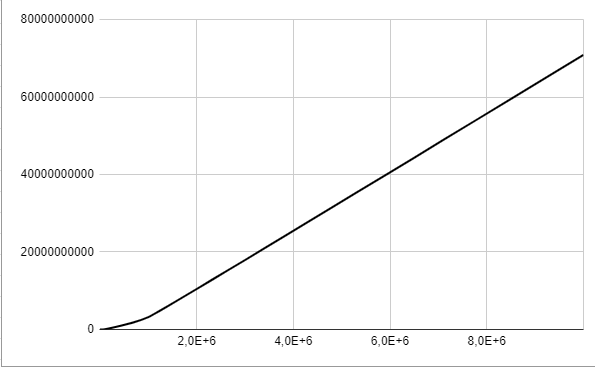
\includegraphics[scale=0.5]{./ressources/tempsexecutiondico.png}
        \caption{Temps d'exécution du programme selon la longueur du tableau}
    \label{fig:temps_exec_dico}
\end{figure}
\par
Depuis le graphe, la courbe est sous forme d'un arc ascendant, on observe que le temps d'exécution évolue de manière linéarithmique avec l'augmentation de la taille du problème, ce qui correspond bien à la complexité théorique calculée auparavant. 

\section{Conclusion}
L'algorithme de la recherche dichotomique propose une complexité optimale pour la recherche dans un tableau, cependant sa dépendance d'une fonction de tri afin de pouvoir fonctionner Quel que soit le tableau donné impacte négativement sa complexité, dans notre l'utilisation d'une fonction de tri dichotomique aura fait passer notre algorithme d'une complexité logarithmique a une complexité linéarithmique. Nous pouvons en conclure que la recherche par dichotomie est effectivement une bonne option, mais qu'afin de pouvoir l'utiliser à son plein potentiel il est nécessaire de l'utiliser sur des tableaux préalablement triés ou accompagné d'une fonction de tri ayant une complexité égale ou meilleur à elle.